\documentclass[aps,pra,notitlepage,amsmath,amssymb,letterpaper,12pt]{revtex4-1}
\usepackage{amsthm}
\usepackage{graphicx}


\newenvironment{problem}[2][Problem]{\begin{trivlist}
\item[\hskip \labelsep {\bfseries #1}\hskip \labelsep {\bfseries #2.}]}{\end{trivlist}}
\newenvironment{solution}{\begin{proof}[Solution]}{\end{proof}}
 

 
\begin{document}
 
\title{Classwork 13: George and Moana but In LaTeX}
\author{Morgan Holve}
\affiliation{MATH 220, Schmid College of Science and Technology, Chapman University}
\date{\today}

\maketitle

\section{Introduction} 
The goal of this is to basically put everything from Classwork 12 and Homework 12 into LaTeX. Allow me to restate everything from those Jupyter notebooks into this:

\vspace{5mm}
We are considering a ball of mass $m$ rolling in a double-well potential (whatever that is) of $V(x) = x^4/4 - x^2/2$. This potential is unaptly called the "sombrero potential" despite its likeness toward stingrays. 

\vspace{5mm}
Taking physics things into account and also remembering that the ball must follow Newton's Second Law, we obtain the equation:
$$m\ddot{x} = f_{\text{hat}}(x) + f_{\text{drag}}(\dot{x}) + f_{\text{drive}}(t) = x - x^3 - \nu \dot{x} + F\cos(\omega t)$$
Which can be split into the system of differential equations:
$$\dot{x}(t) = y(t)$$
$$m\dot{y}(t) = -\nu y(t) + x(t) - x^3(t) + F\cos(\omega t)$$
Here, we will solve these using the Runge-Kutta 4th Order method outlined in the past two classworks, taking $m = 1$, $\omega = 1$ and $\nu = .25$. We'll graph our results and then see what everything means. \par
\noindent
Reminder of the method:
$u_{k+1} = u_k + (K_1 + 2K_2 + 2K_3 + K_4)/6$, 
   
   with
   
   $K_1 = \Delta t\,f[t_k,u_k]$, 
   
   $K_2 = \Delta t\, f[t_k + \Delta t/2, u_k + K_1/2]$, 
   
   $K_3 = \Delta t\, f[t_k + \Delta t/2, u_k + K_2/2]$, 
   
   $K_4 = \Delta t\,f[t_k + \Delta t, u_k + K_3]$  
   

\section{Implementation}
We solved the differential equation each for different $F$ values and initial conditions.

\subsection{Varying Intial Conditions}
When our code was implemented, the following figures were produced for the different initial conditions.

\begin{figure}[h!] 
  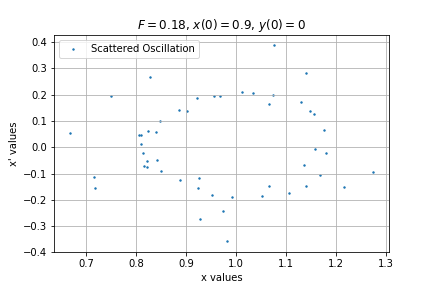
\includegraphics[width=0.4\textwidth]{frame02.jpg}  
  \caption{Initial Conditions: $F = 0.18$, $t\in[0,2\pi\, 50]$, with $x(0) = 0.9$ and $y(0) = 0$; Scatter Plot}
  \label{fig:figlabel}
\end{figure}

\begin{figure}[h!] % h forces the figure to be placed here, in the text
  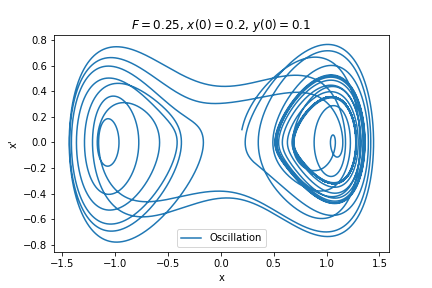
\includegraphics[width=0.4\textwidth]{frame04.jpg}  % if pdflatex is used, jpg, pdf, and png are permitted
  \caption{Initial Conditions: $F = 0.25$, $t\in[0,2\pi\, 50]$, with $x(0) = 0.2$ and $y(0) = 0.1$}
  \label{fig:figlabel}
\end{figure}

\section{Analysis}
Now, what do these graphs mean? To do this, we look at the relative density of the lines on each side of the graph. For Figure 1, we see that both the left and right sides of the figure are balanced, meaning the ball moved uniformly and evenly in between the wells. However, in Figure 2, we see that the right side is obviously favored over the left, meaning the ball spend more time in the rightmost well rather than the left. \par
\noindent
For your viewing pleasure, here is the Moana graph because I'm a little obsessed with it.
\begin{figure}[h!] % h forces the figure to be placed here, in the text
  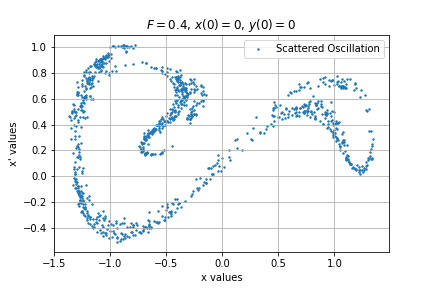
\includegraphics[width=0.4\textwidth]{frame03.jpg}  % if pdflatex is used, jpg, pdf, and png are permitted
  \caption{See the light as it shines on the sea, it calls me. And no one knows how far it goes. If the wind in my sail on the sea stays behind me, I know one day I'll find the way.}
  \label{fig:figlabel}
\end{figure}
\end{document}
